% arara: xelatex
% arara: xelatex
% arara: xelatex


% options:
% thesis=B bachelor's thesis
% thesis=M master's thesis
% czech thesis in Czech language
% english thesis in English language
% hidelinks remove colour boxes around hyperlinks

\documentclass[thesis=B,english]{FITthesis}[2012/10/20]

% \usepackage[utf8]{inputenc} % LaTeX source encoded as UTF-8
% \usepackage[latin2]{inputenc} % LaTeX source encoded as ISO-8859-2
% \usepackage[cp1250]{inputenc} % LaTeX source encoded as Windows-1250

\usepackage{graphicx} %graphics files inclusion
% \usepackage{subfig} %subfigures
% \usepackage{amsmath} %advanced maths
% \usepackage{amssymb} %additional math symbols

\usepackage{dirtree} %directory tree visualisation

% % list of acronyms
% \usepackage[acronym,nonumberlist,toc,numberedsection=autolabel]{glossaries}
% \iflanguage{czech}{\renewcommand*{\acronymname}{Seznam pou{\v z}it{\' y}ch zkratek}}{}
% \makeglossaries

% % % % % % % % % % % % % % % % % % % % % % % % % % % % % % 
% EDIT THIS
% % % % % % % % % % % % % % % % % % % % % % % % % % % % % % 

\department{Department of Software Engeeniring}
\title{StudyPad - Android Client}
\newcommand{\appname}{StudyPad}
\authorGN{Roman} %author's given name/names
\authorFN{Levinzon} %author's surname
\author{Roman Levinzon} %author's name without academic degrees
\authorWithDegrees{Roman Levinzon} %author's name with academic degrees
\supervisor{Ing. Miroslav Bal{\'i}k, Ph.D}
\acknowledgements{THANKS (remove entirely in case you do not with to thank anyone)}
\abstractEN{StudyPad is a combination of note-taking service and a social network, aimed to help students to memorise different pieces of information.  The goal of this thesis is to develop an application for Android OS which will serve as client. This text acknowledges existing solutions, contains domain and requirements analysis, description and choise of application's architecture and it's implementation}


\abstractCS{StudyPad je kombinace slu{\v z}by pro pori{\v z}ovan{\' i} pozn{\'a}mek a soc{\'i}{\'a}ln{\'i} s{\'i}t{\v e} s c{\'i}lem  pomoci studentum zapamatovat si ruzn{\'e} informace. C{\'i}lem pr{\'a}ce je vyvinout aplikaci pro OS Android, kter{\'a} bude slou{\v z}it jako klient. Tento text uzn{\'a}v{\'a} st{\'a}vaj{\' i}c{\'i} {\v r}e{\v s}en{\'i}, obsahuje anal{\'y}zu dom{\'e}n a po{\v z}adavku, popis a v{\'y}b{\v e}r architektury aplikace a jej{\'i} implementace}
\placeForDeclarationOfAuthenticity{Prague}
\keywordsCS{Android, Kotlin, MVVM}
\keywordsEN{Android, Kotlin, MVVM}
\declarationOfAuthenticityOption{1} %select as appropriate, according to the desired license (integer 1-6)
% \website{http://site.example/thesis} %optional thesis URL


\begin{document}

% \newacronym{CVUT}{{\v C}VUT}{{\v C}esk{\' e} vysok{\' e} u{\v c}en{\' i} technick{\' e} v Praze}
% \newacronym{FIT}{FIT}{Fakulta informa{\v c}n{\' i}ch technologi{\' i}}

\setsecnumdepth{part}
\chapter{Introduction}

Each year, our smartphones get smarter and mobile applications - more advanced. Arrival of smartphones and mobile applications completely changed our way. of life, made it easier and it is hard to come up with the single aspect of it, which was not improved by some or the a other application. They are everywhere: helping us to navigate in our neighbourhood, keeping up to date with latest news, helping us to stay in touch with our loved ones, stay  fit and healthy and more. And some of the most popular applications tend to teach us something new.	

Educational apps are one of the most popular apps on both mobile platforms (iOS and Android). Many of them use the so-called flash card system in the study process - displaying small pieces of information one after another so the user could memorise it more easily. However, most of these services are fairly limited in terms of what the are trying to teach and some of the greatest  features are scattered across different applications. \appname\ wants to give its users freedom in what they want to learn and deliver convenient environment to make study process even more easier

\subsection{\appname\ service}
\appname\ is a combination of a note taking service and a social network. This service is focused primarily on students and it aims to get rid of the boundaries of what it can teach - because users will be able to create teaching materials themselves and share it with each other.

The basis of \appname\ is such concepts as Notebook. Notebook is simply a collection of notes united by one theme. This may be a subject in school, a language that you would like to learn, or a set of questions that you can hear at the job interview. Note, in turn, is a part of the notebook and represents a single piece information that has a name and content. Note can be interpreted as a question and answer, or a term and its definition.

Each user has his own space where he can create, store and edit his notebooks (Further Library) and then use as a basis for various tests and exercises to quickly memorise information from a notebook using the familiar flash card system

\appname\ also allows users to easily share these notebooks with each other. Each notebook can be published, thereby making it available for viewing and downloading to other users.
The publication process is to provide additional information about the notebook, including its name, optional description, topic and optional tags that serve to narrow the topic. All this data, including the author's school, will then be used in the process of searching and filtering - which will facilitate the search for the necessary materials. There is also the ability to quickly send a notebook using the links. In this case, if the notepad has not yet been published, its published version will be created with a minimum of details and excluded from the search results, making it accessible only using link until all details nedeed are provided, link to the Published version will be sent otherwise


The author of the notebook reserves the right to make edits/corrections the notebook located in the shared space by editing the his local notebook. Other users (hereinafter subscribers) in turn can save the Published notebook to their library, discuss this notebook with other users, or suggest the author changes or corrections to improve the content inside. By saving Published notebook to his library, subscriber will be able to make any local changes as he sees fit and use it as normal. Subscribers will be notified about any updates to the Published Notebook so that they can apply changes to their local versions locally, though any local changes will be deleted. The author of the notebook, in turn, will be notified of such activities as: suggestion or correction of content and new comments left by subscribers

\setsecnumdepth{all}
\newpage
\chapter{Analysis}

This chapter contains \appname\ application analysis with the goal to identify requirements and how it is compared with its rivals

// TODO Component diagram

\section{System description}
 \appname\ system follows client-server software architecture. Server part is presented by REST API thats is developed using Spring framework. Client part consists of  client applications for several platforms: Android, iOS and Web. Main task of this thesis is to deliver an Android application. iOS  application is developed as a part subject called BI-IOS and hence, has some limitations in its implementation. Web client is being developed alongside the Android one is serves as Admin Panel for the server which allows to modify certain data without dealing with the server directly.
 
 
 
 The detailed structure of the Android client structure and its connection with other components are presented in the component diagram bellow. It will be connected with Facebook SDK and Google Auth SDK to provide options for user to login and some minimal setup of Firebase SDK to enable analytics and crash reporting functionality 


\section{Domain Description}
Class diagram bellow represents Domain Model of the application, it provides visual representation of Entities and relations between them. Design is based on the entities used on server-side

\begin{figure}[t]
	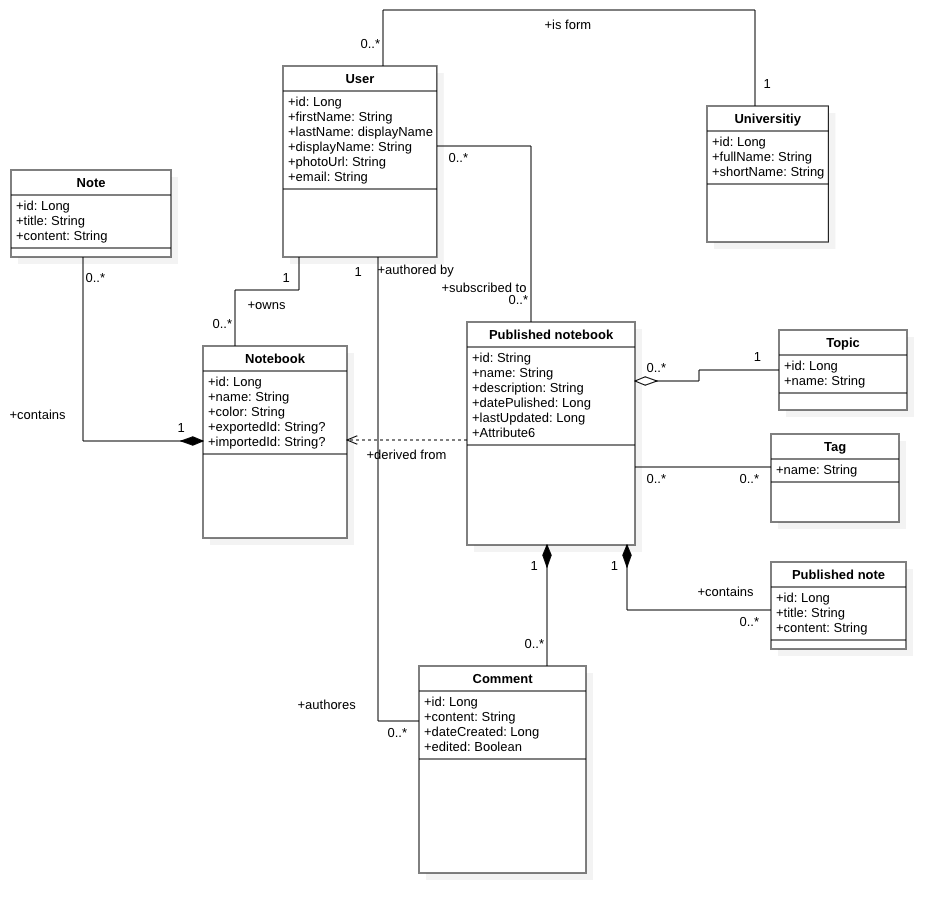
\includegraphics[scale=0.4]{Domain}
\end{figure}

\subsection{User}
	User entity represents someone who have completed registration flow using one of the client app. This entity contains such properties as: firstName, lastName, email, password, university. Due to the fact, that \appname\ provides several ways for user to authorize, some of the properties will either come from the user's input or from the 3rd party API ( Google or Facebook ).

	
\subsection{Note}
	Note represent a single piece of information. It consists of two properties: title and content. These can be described as term and defenition or question and answer. Every note must be assigned to one of the notebooks, hence theres a 1:N relation
\subsection{Notebook}
	Notebook is one of the main entities used in the application flow, and  can be created by an authenticated user. Soul purpose of the Notebook is to store Notes and serve as a source for Shared Notebook. Properties name and color are used to help users distinct between different Notebooks
	
	
\subsection{University}
University represents school, where User can assign himself as a student during registration flow. It is used to unite users from the same schools, so they could faster find content they are looking for.

\subsection{Published Notebook}
Published Notebook represents a shareable content. It can be created by user, based on one of his/her notebooks by providing some additional details:
name, optional description,  Topic and optional set of Tags. All these details are later used for Search flow to optimize searching results.

\subsection{Published Note}
Published Note represent the note inside of the Published Notebook and  contains the exact same properties as usual note

\subsection{Topic}
Topic represents main topic or subject of the Published Notebook. Topic consist of only one property: name
\subsection{Tag}
Tag is us short label thats attached to the Published Notebook. It is mainly  used to narrow the topic or school. Tag has only one property - it's actual value stored as name

\subsection{Comment}
Users can comment on published notebooks. Most of the properties are assigned automatically, the only exception is content which is property that represents the body of the comment. All other properties are assigned automatically and can not be changed

\section{Android Platform}




\newpage
\section{Requirements}
It is important to establish all functional and non-functional requirements for \appname. Section bellow contains all requirements designed before the start
of the development

\subsection{Functional requirements}
\bigskip
\textbf{User Authentication}
\begin{itemize}
	\item \textbf{F1: Registration/Login using email} Access to \appname\ is possible by creating an account using email address/password combination.
	\item \textbf{F2: Registration/Login using Facebook} User will be able to use his/her Facebook account to access \appname.
	\item \textbf{F3: Registration/Login using Google} User will be able to use his/her Google account to access \appname.
	\item \textbf{F4: Store OAuth token} API Authentication Token will be stored in device memory.
	\item \textbf{F5: Token refreshment} API Token will be refreshed when needed, so user won't have to login again.
	\item \textbf{F6: University selection} As a part of user registration flow, user will be able to select his/her university.
\end{itemize}
\bigskip
\textbf{Library Management (Notes \& Notebooks)}
\begin{itemize}
	\item \textbf{F7: Notebook creation} User will be able to create new notebooks with the name he/she choose.
	\item \textbf{F8: Notebook deletion} User will be able to delete existing notebooks.
	\item \textbf{F9: Notebook name edition} User will be able to edit notebooks names.
	\item \textbf{F10: Note creation} User will be able to create a note with specific title and content.
	\item \textbf{F11: Note edition} User will be able to edit existing note, or completely delete it.
	\item \textbf{F12: Show Notebooks} : User will be able to view all the notebooks he/she created.
	\item \textbf{F13: Show Notes}: By clicking on notebook item, user will be able to view the list of notes that are assigned to this notebook.
\end{itemize}

\bigskip
\textbf{Sharing Hub}
\begin{itemize}
	\item \textbf{F14: View published notebooks} User will be able to view notebooks published by other users.
	\item \textbf{F15: Search through published books} User will be able to search through the published notebooks by applying different filters (such as author, university and subject/topic).
	\item \textbf{F16: Browse through published notebook} User will be able to see notes inside the notebook that's been published.
	\item \textbf{F17: View comments} User will be able to view others users comments discussing a notebook that's been published.
	\item \textbf{F18: Leave a comment} User can comment on other user published notebook.
	\item \textbf{F19: Delete a comment} Application will let user to delete his/her comment.
	\item \textbf{F20: Save published notebook} User will be able to save published notebook to his/her library.
	\item \textbf{F21: Publish notebook} User will be able to publish his/her notebook.
	\item \textbf{F22: Update published notebook} Author of the published notebook will be able to update its information.
	\item \textbf{F23: Delete published notebook} Author of the published notebook will be able to delete the his/her notebook from shared space.
	\item \textbf{F24: Share notebook} User will be able to share his/her notebook by generating a deep-link.
 \end{itemize}

\bigskip
\textbf{Study Hub}
\begin{itemize}
	\item \textbf{F25: Start a basic self-check} User will be able to use an interactive way to look through his/her notes
	\item \textbf{F26: Start a written test} User will be able to participate in a written test based on one of notebooks to test his/her knowledge
	\item \textbf{F27: Start a quiz} User will be able to participate in quiz challenge that will be based on one of his/her notebooks
	
\end{itemize}

\bigskip
\textbf{Settings}
\begin{itemize}
	\item \textbf{F28: View Profile Information} User will be able to view his/her profile information such as first name, last name and  university.
	\item \textbf{F29: Edit Profile Information} User will be able to edit his/her profile information.
	\item \textbf{F30: Logout} User will be able to logout from the application.
\end{itemize}


\subsection{Non-functional requirements}

\begin{itemize}
  \item \textbf{N1: Native Android application}  Application will be written using native Android SDK.
  \item \textbf{N2: Android Version} Application minimal SDK version must be low enough to support as many devices as possible and high enough to use most applicable  Android APIs considering other functional and non-functional requirements.
  \item \textbf{N3: Material Design} Application user interface will follow latest Material design guidelines and best practises.
  \item \textbf{N4: Scalable app architecture} Application's architecture must be scalable and easy testable.
  \item \textbf{N5: Tablet \& Phone support} Application GUI must be well suited for multiple screen sizes.
  \item \textbf{N6: App Localization} Application will be able to adapt to different languages based on user locale
\end{itemize}


\newpage

\section{Existing solutions}

There are several apps out there, whose goal is similar to \appname. However, most of the solutions are limited to learning languages and have limited sharing and discovering options. Table bellow shows requirements comparison such apps

\bigskip

\begin{tabular}{|l|l|l|l|}
\hline
\textbf{\begin{tabular}[c]{@{}l@{}}Application\\ Requirement\end{tabular}} & \multicolumn{1}{c|}{\textbf{Quizlet}} & \multicolumn{1}{c|}{\textbf{Cram}} & \multicolumn{1}{c|}{\textbf{TinyCards}} \\ \hline
\textbf{F1}                                                                & Present                               & Present                            & Present                                 \\ \hline
\textbf{F2}                                                                & Present                               & Present                            & Present                                 \\ \hline
\textbf{F3}                                                                & Present                               & Present                            & Present                                 \\ \hline
\textbf{F4}                                                                & Present                               & Present                            & Present                                 \\ \hline
\textbf{F5}                                                                & Present                               & Present                            & Present                                 \\ \hline
\textbf{F6}                                                                & Absent                                & Absent                             & Absent                                  \\ \hline
\textbf{F7}                                                                & Present                               & Present                            & Present                                 \\ \hline
\textbf{F8}                                                                & Present                               & Present                            & Present                                 \\ \hline
\textbf{F9}                                                                & Present                               & Present                            & Present                                 \\ \hline
\textbf{F10}                                                               & Present                               & Present                            & Present                                 \\ \hline
\textbf{F11}                                                               & Present                               & Present                            & Present                                 \\ \hline
\textbf{F12}                                                               & Present                               & Present                            & Present                                 \\ \hline
\textbf{F13}                                                               & Present                               & Present                            & Present                                 \\ \hline
\textbf{F14}                                                               & Absent                                & Absent                             & Present                                 \\ \hline
\textbf{F15}                                                               & Limited                               & Limited                            & Limited                                 \\ \hline
\textbf{F16}                                                               & Present                               & Present                            & Present                                 \\ \hline
\textbf{F17}                                                               & Absent                                & Absent                             & Absent                                  \\ \hline
\textbf{F18}                                                               & Absent                                & Absent                             & Absent                                  \\ \hline
\textbf{F19}                                                               & Absent                                & Absent                             & Absent                                  \\ \hline
\textbf{F20}                                                               & Present                               & Limited                            & Limited                                 \\ \hline
\textbf{F21}                                                               & Limited                               & Limited                            & Limited                                 \\ \hline
\textbf{F22}                                                               & Present                               & Present                            & Present                                 \\ \hline
\textbf{F23}                                                               & Present                               & Present                            & Present                                 \\ \hline
\textbf{F24}                                                               & Present                               & Limited                            & Limited                                 \\ \hline
\textbf{F25}                                                               & Present                               & Present                            & Limited                                 \\ \hline
\textbf{F26}                                                               & Present                               & Present                            & Limited                                 \\ \hline
\textbf{F27}                                                               & Present                               & Present                            & Limited                                 \\ \hline
\textbf{F28}                                                               & Present                               & Present                            & Limited                                 \\ \hline
\textbf{F29}                                                               & Limted                                & Limted                             & Limited                                 \\ \hline
\textbf{F30}                                                               & Present                               & Present                            & Limited                                 \\ \hline
\end{tabular}

\bigskip
\subsection{Quzlet - Key differences}

\textbf{Quizlet} is primarily used for learning languages, from where most of the limitations come from. Closest analogy to Notebook there is Study set with Terms inside. This makes it easier for tests generation, but limits user when he/she is trying to learn anything other than new words



\begin{itemize}
	\item \textbf{Publishing}: Content publishing process is very different to what \appname\ is trying to achieve. All study sets are visible to other users by default, which makes it hard, if not impossible, to distinct between local and shared published set.
	\item \textbf{Importing}: Importing flow allows user to either copy or save study set to a specific folder. This flow may confuse some of the users, because only copy allows actually add set to user library and modify it. Saving study set to the specific folder only saves the link to it and splits library management in 2 parts.
	\item \textbf{Discovering:} This limitation comes from the fact, that Quizlet is an app for language learners. As a consequence, the only distinctions between Study sets are its name and a language. These are the only 2 options available for filtering published study sets.

\end{itemize}

\subsection{Cram - Key differences}
\textbf{Cram} is very similar to Quizlet but feels much more outdated in terms of UX and brings some sharing limitations to the table.

\begin{itemize}
	\item  \textbf{Publishing:} Content publishing is similar to Quizlet - All sets are either visible by other users or not. Sharing a deep-link to a single study set was not functional at the time of writing this section
	\item \textbf{Discovering} Searching for content in Cram is even more limited comparing to Quizlet, only name of the study set is used
	\item \textbf{Importing} Library management here is splitted in 3 parts: User personal sets, Favourite sets, and Recently studied. When searching, there is no way to save published study set to personal library, it can only be automatically saved to Recent section, or manually added to Favourites. This makes it impossible to make local edits
\end{itemize}

\subsection{TinyCards - Key Differences}

\textbf{TinyCards} is app made by Duolingo, one of the biggest app for learning languages. TinyCard is meant to be more generic as it offers users to create custom study sets, often not limited to languages
	\begin{itemize}
		\item \textbf{Importing:} Similar to Cram, it is not possible to edit the study set user have downloaded and saved to his library
		\item \textbf{Challenges:} Tests for user are generated automatically and there is no way to choose test type
	\end{itemize}
	
\newpage

\chapter{Design}
\section{Wireframes}
\section{Application architecture}
\section{Platform-specific model}
\section{Main sequence diagrams}

\chapter{Implementation}
\section{Choice of technologies}
\section{Component diagram}
\section{Installation}


\chapter{Testing}


\setsecnumdepth{part}
\chapter{Conclusion}


\bibliographystyle{iso690}
\bibliography{mybibliographyfile}

\setsecnumdepth{all}
\appendix

\chapter{Acronyms}
% \printglossaries
\begin{description}
	\item[GUI] Graphical user interface
	\item[XML] Extensible markup language
\end{description}


\chapter{Contents of enclosed CD}

%change appropriately

\begin{figure}
	\dirtree{%
		.1 readme.txt\DTcomment{the file with CD contents description}.
		.1 exe\DTcomment{the directory with executables}.
		.1 src\DTcomment{the directory of source codes}.
		.2 wbdcm\DTcomment{implementation sources}.
		.2 thesis\DTcomment{the directory of \LaTeX{} source codes of the thesis}.
		.1 text\DTcomment{the thesis text directory}.
		.2 thesis.pdf\DTcomment{the thesis text in PDF format}.
		.2 thesis.ps\DTcomment{the thesis text in PS format}.
	}
\end{figure}

\end{document}
